\section{Problem specification}

\begin{figure}[ht]
    \centering
    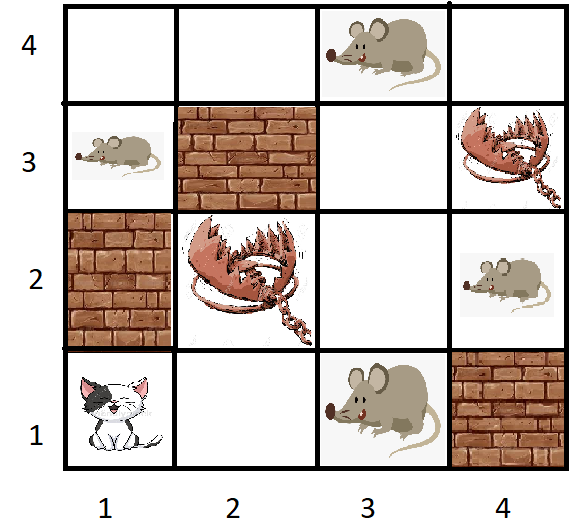
\includegraphics[width=.5\linewidth]{fig/A3/cat_06.png}
    \caption{Example instance of the cat-mouse world}
    \label{fig:overview}
\end{figure}


The world is represented by 16 rooms (4×4) or extended to 36 rooms (6x6). Each room is connected to others through walkways (no rooms are connected diagonally). The knowledge-based agent is a cat which starts from room (1, 1). The goal of the cat is to get rid of the mice: by eating them or by dropping them on traps. After each mouse the cat receives a reward. The walls block the path of the cat, forcing it to go around. The trap kills the animal that lands on it, however it can be used only once. Figure \ref{fig:overview} shows an example instance of the problem.
